%                                                                 aa.dem
% AA vers. 9.1, LaTeX class for Astronomy & Astrophysics
% demonstration file
%                                                       (c) EDP Sciences
%-----------------------------------------------------------------------
%
% \documentclass[referee]{aa} % for a referee version
%\documentclass[onecolumn]{aa} % for a paper on 1 column  
%\documentclass[longauth]{aa} % for the long lists of affiliations 
%\documentclass[letter]{aa} % for the letters 
%\documentclass[bibyear]{aa} % if the references are not structured 
%                              according to the author-year natbib style

%

\documentclass{aa}  

%
\usepackage{graphicx}
\usepackage{amsmath,amsfonts,amssymb}
\usepackage{natbib}
\usepackage{tabularx}
\usepackage{collcell}
\usepackage{array}
\usepackage{booktabs}

%%%%%%%%%%%%%%%%%%%%%%%%%%%%%%%%%%%%%%%%
\usepackage{txfonts}
\usepackage{xcolor}
\usepackage{blindtext}
%%%%%%%%%%%%%%%%%%%%%%%%%%%%%%%%%%%%%%%%
% \usepackage[options]{hyperref}
% To add links in your PDF file, use the package "hyperref"
% with options according to your LaTeX or PDFLaTeX drivers.
\usepackage{float}
%\usepackage{stfloats}
\usepackage{dblfloatfix}
\usepackage{afterpage}
\usepackage{ifthen}
\usepackage[morefloats=12]{morefloats}

\usepackage{placeins}
\usepackage{multicol}
%\usepackage[breaklinks,colorlinks,citecolor=blue]{hyperref}
\bibpunct{(}{)}{;}{a}{}{,}
\usepackage[switch]{lineno}
\definecolor{linkcolor}{rgb}{0.6,0,0}
\definecolor{citecolor}{rgb}{0,0,0.75}
\definecolor{urlcolor}{rgb}{0.12,0.46,0.7}
\usepackage[breaklinks, colorlinks, urlcolor=urlcolor,
linkcolor=linkcolor,citecolor=citecolor,pdfencoding=auto]{hyperref}
\hypersetup{linktocpage}
\usepackage{bold-extra}

%Planck style file, to be used with A&A style to produce Planck papers for publication.
%
% version 28 September 2010 --- useful macros --- CRL
% version 17 October 2010   --- first cut at important instrument values, from Daniele Mennella and
%                               Francois Bouchet, 13 October 2010 --- CRL
% version 18 October 2010   --- LFI FWHM changed to one value per feed, rather than M & S separately
%                               LFI FWHM uncertainties added for individual feeds.  Corrections made
%                               to LFI values. --- Andrea Zacchei
% version 24 October 2010   --- added to and corrected definitions.  No changes made to instrument
%                               quantities. --- CRL 
% version 31 October 2010   --- added definition of \muKHz. --- CRL
%
% version 15 November 2010  --- fixed conflict with aa.cls in definition of \endtable
%                               by naming the command below "\endPlancktable".  See section
%                               13.16 of the Style Guide.
%
% version 06 December 2010  --- Set up names with and without units.
%                               Add \allearlypapers command to ensure that all early papers are
%                               included in the reference list.
%                               Define macro for the name of the 4He JT cooler.
%
% version 07 December 2010  --- removed extraneous "planck2011-1.2" entry in \allearlypapers
%
% version 12 December 2010  --- added \endPlancktablewide command to set tablenotes to the full
%                               page width in the \begin{table*}...\end{table*} environment when
%                               the ``twocolumn'' option is specified in the \documentclass command.
%                               (It would be more elegant to extract the appropriate width from the
%                               aa.cls system at the time of execution, but that is buried more
%                               deeply in the system than I investigated.)
%
% version 05 January 2011   --- added unit \MJysr.  HFI performance values updated per FRB email
%                               01/05/2011 02:38-0800, and Brendan Crill email 01/05/2011 18:08 -0800.
%
% version 06 January 2011   --- changed \scriptscriptstyle primes to \scriptstyle, to better match the
%                               tx fonts used by A&A.
%
% version 07 January 2011   --- modified \allearlypapers to correspond with final early paper list.  
%                               Fixed 545 GHz center frequency.
%
% version 07 January 2011b  --- changed LFI white-noise sensitivity numbers to correct problem with units
%
% version 05 July 2011      --- added \Msol and \Lsol to get the symbols for solar mass and luminosity.
%                               Deleted previous definitions of \solar and \sol, which were equivalent
%                               to the new \Msol.
%
% version 16 August 2011    --- changed comments on \endPlancktable and \endPlancktablewide for clarity
%
% version 11 September 2011 --- changed definition of \tablenote to make footnote labels italic, as per A\&A
%
% version 26 April 2011     --- changed definition of \Planck to agree with what is said in the Style Guide (!)
%
% version 04 Dec 2013       --- included 2013 results references
%
% version 17 Jan 2014       --- included fix to bibtex file v4.3, i.e. \providecommand{\sorthelp}[1]{}
%
% version 26 Jul 2014       --- fixed incompatibility problem with aa.cls v8.0 and v8.2.  v8.2 should now be used
%                               for all Planck papers.
%                           --- fixed problem in definition of "\all2013resultspapers" that introduced a blanck
%                               into the reference to p06b.
%                           --- removed all the parameter definition stuff at the end.  We weren't using it, and
%                               it took up a lot of space.
%
% version 28 Jan 2015       --- added "\alltwentyfiftennresultspapers" and corrected "\all2013resultspapers" to
%                               "\all20thirteenresultspapers",
%
% Usage:  after the \documentclass[traditabstract]{aa} command in the La\TeX\ input file,
%         add this command:      \input Planck.tex


\def\setsymbol#1#2{\expandafter\def\csname #1\endcsname{#2}}
\def\getsymbol#1{\csname #1\endcsname}

%-----------------------------------------------------------------------
% Planck
%-----------------------------------------------------------------------
\def\Planck{\textit{Planck}}

%-----------------------------------------------------------------------
% The Planck Helium-4 JT cooler
%-----------------------------------------------------------------------
\def\HeJT{$^4$He-JT}

%-----------------------------------------------------------------------
% To include all Planck Early Results papers in the reference lists
%-----------------------------------------------------------------------
\def\allearlypapers{\nocite{planck2011-1.1, planck2011-1.3, planck2011-1.4, planck2011-1.5, planck2011-1.6, planck2011-1.7, planck2011-1.10, planck2011-1.10sup, planck2011-5.1a, planck2011-5.1b, planck2011-5.2a, planck2011-5.2b, planck2011-5.2c, planck2011-6.1, planck2011-6.2, planck2011-6.3a, planck2011-6.4a, planck2011-6.4b, planck2011-6.6, planck2011-7.0, planck2011-7.2, planck2011-7.3, planck2011-7.7a, planck2011-7.7b, planck2011-7.12, planck2011-7.13}}

%-----------------------------------------------------------------------
% To include all Planck 2013 Results papers in the reference lists
%-----------------------------------------------------------------------
\def\alltwentythirteenresultspapers{\nocite{planck2013-p01, planck2013-p02, planck2013-p02a, planck2013-p02d, planck2013-p02b, planck2013-p03, planck2013-p03c, planck2013-p03f, planck2013-p03d, planck2013-p03e, planck2013-p01a, planck2013-p06, planck2013-p03a, planck2013-pip88, planck2013-p08, planck2013-p11, planck2013-p12, planck2013-p13, planck2013-p14, planck2013-p15, planck2013-p05b, planck2013-p17, planck2013-p09, planck2013-p09a, planck2013-p20, planck2013-p19, planck2013-pipaberration, planck2013-p05, planck2013-p05a, planck2013-pip56, planck2013-p06b, planck2013-p01a}}

%-----------------------------------------------------------------------
% To include all Planck 2015 Results papers in the reference lists
%-----------------------------------------------------------------------
\def\alltwentyfifteenresultspapers{\nocite{planck2014-a01, planck2014-a03, planck2014-a04, planck2014-a05, planck2014-a06, planck2014-a07, planck2014-a08, planck2014-a09, planck2014-a11, planck2014-a12, planck2014-a13, planck2014-a14, planck2014-a15, planck2014-a16, planck2014-a17, planck2014-a18, planck2014-a19, planck2014-a20, planck2014-a22, planck2014-a24, planck2014-a26, planck2014-a28, planck2014-a29, planck2014-a30, planck2014-a31, planck2014-a35, planck2014-a36, planck2014-a37, planck2014-ES}}

%-----------------------------------------------------------------------
% Tables
%-----------------------------------------------------------------------
\newbox\tablebox    \newdimen\tablewidth
\def\leaderfil{\leaders\hbox to 5pt{\hss.\hss}\hfil}
%
% use the following definition of \endPlancktable for ApJ style notes to tables, set to the 
%         width of the table
% \def\endPlancktable{\tablewidth=\wd\tablebox 
%
% use the following definitions of \endPlancktable and \endPlancktablewide for A&A style notes 
% set to one-column  or full-page width, respectively
\def\endPlancktable{\tablewidth=\columnwidth 
    $$\hss\copy\tablebox\hss$$
    \vskip-\lastskip\vskip -2pt}
\def\endPlancktablewide{\tablewidth=\textwidth 
    $$\hss\copy\tablebox\hss$$
    \vskip-\lastskip\vskip -2pt}
\def\tablenote#1 #2\par{\begingroup \parindent=0.8em
    \abovedisplayshortskip=0pt\belowdisplayshortskip=0pt
    \noindent
    $$\hss\vbox{\hsize\tablewidth \hangindent=\parindent \hangafter=1 \noindent
    \hbox to \parindent{$^#1$\hss}\strut#2\strut\par}\hss$$
    \endgroup}
\def\doubleline{\vskip 3pt\hrule \vskip 1.5pt \hrule \vskip 5pt}

%-----------------------------------------------------------------------
% useful macros
%-----------------------------------------------------------------------
%
\def\L2{\ifmmode L_2\else $L_2$\fi}
%
\def\dtt{\Delta T/T}
\def\DeltaT{\ifmmode \Delta T\else $\Delta T$\fi}
\def\deltat{\ifmmode \Delta t\else $\Delta t$\fi}
\def\fknee{\ifmmode f_{\rm knee}\else $f_{\rm knee}$\fi}
\def\Fmax{\ifmmode F_{\rm max}\else $F_{\rm max}$\fi}
%
\def\solar{\ifmmode{\rm M}_{\mathord\odot}\else${\rm M}_{\mathord\odot}$\fi}
\def\Msolar{\ifmmode{\rm M}_{\mathord\odot}\else${\rm M}_{\mathord\odot}$\fi}
\def\Lsolar{\ifmmode{\rm L}_{\mathord\odot}\else${\rm L}_{\mathord\odot}$\fi}
%
\def\inv{\ifmmode^{-1}\else$^{-1}$\fi}
\def\mo{\ifmmode^{-1}\else$^{-1}$\fi}
\def\sup#1{\ifmmode ^{\rm #1}\else $^{\rm #1}$\fi}
\def\expo#1{\ifmmode \times 10^{#1}\else $\times 10^{#1}$\fi}
%
\def\,{\thinspace}
\def\lsim{\mathrel{\raise .4ex\hbox{\rlap{$<$}\lower 1.2ex\hbox{$\sim$}}}}
\def\gsim{\mathrel{\raise .4ex\hbox{\rlap{$>$}\lower 1.2ex\hbox{$\sim$}}}}
\let\lea=\lsim
\let\gea=\gsim
\def\simprop{\mathrel{\raise .4ex\hbox{\rlap{$\propto$}\lower 1.2ex\hbox{$\sim$}}}}
%
\def\deg{\ifmmode^\circ\else$^\circ$\fi}
\def\pdeg{\ifmmode $\setbox0=\hbox{$^{\circ}$}\rlap{\hskip.11\wd0 .}$^{\circ}
          \else \setbox0=\hbox{$^{\circ}$}\rlap{\hskip.11\wd0 .}$^{\circ}$\fi}
\def\arcs{\ifmmode {^{\scriptstyle\prime\prime}}
          \else $^{\scriptstyle\prime\prime}$\fi}
\def\arcm{\ifmmode {^{\scriptstyle\prime}}
          \else $^{\scriptstyle\prime}$\fi}
\newdimen\sa  \newdimen\sb
\def\parcs{\sa=.07em \sb=.03em
     \ifmmode \hbox{\rlap{.}}^{\scriptstyle\prime\kern -\sb\prime}\hbox{\kern -\sa}
     \else \rlap{.}$^{\scriptstyle\prime\kern -\sb\prime}$\kern -\sa\fi}
\def\parcm{\sa=.08em \sb=.03em
     \ifmmode \hbox{\rlap{.}\kern\sa}^{\scriptstyle\prime}\hbox{\kern-\sb}
     \else \rlap{.}\kern\sa$^{\scriptstyle\prime}$\kern-\sb\fi}
%
\def\ra[#1 #2 #3.#4]{#1\sup{h}#2\sup{m}#3\sup{s}\llap.#4}
\def\dec[#1 #2 #3.#4]{#1\deg#2\arcm#3\arcs\llap.#4}
\def\deco[#1 #2 #3]{#1\deg#2\arcm#3\arcs}
\def\rra[#1 #2]{#1\sup{h}#2\sup{m}}
%
\def\page{\vfill\eject}
\def\dots{\relax\ifmmode \ldots\else $\ldots$\fi}
%
%-----------------------------------------------------------------------
% units
%-----------------------------------------------------------------------
%
\def\WHzsr{\ifmmode $W\,Hz\mo\,sr\mo$\else W\,Hz\mo\,sr\mo\fi}
\def\mHz{\ifmmode $\,mHz$\else \,mHz\fi}
\def\GHz{\ifmmode $\,GHz$\else \,GHz\fi}
\def\mKs{\ifmmode $\,mK\,s$^{1/2}\else \,mK\,s$^{1/2}$\fi}
\def\muKs{\ifmmode \,\mu$K\,s$^{1/2}\else \,$\mu$K\,s$^{1/2}$\fi}
\def\muKRJs{\ifmmode \,\mu$K$_{\rm RJ}$\,s$^{1/2}\else \,$\mu$K$_{\rm RJ}$\,s$^{1/2}$\fi}
\def\muKHz{\ifmmode \,\mu$K\,Hz$^{-1/2}\else \,$\mu$K\,Hz$^{-1/2}$\fi}
\def\MJysr{\ifmmode \,$MJy\,sr\mo$\else \,MJy\,sr\mo\fi}
\def\MJysrmK{\ifmmode \,$MJy\,sr\mo$\,mK$_{\rm CMB}\mo\else \,MJy\,sr\mo\,mK$_{\rm CMB}\mo$\fi}
\def\microns{\ifmmode \,\mu$m$\else \,$\mu$m\fi}
\def\micron{\microns}
\def\muK{\ifmmode \,\mu$K$\else \,$\mu$\hbox{K}\fi}
\def\microK{\ifmmode \,\mu$K$\else \,$\mu$\hbox{K}\fi}
\def\muW{\ifmmode \,\mu$W$\else \,$\mu$\hbox{W}\fi}
\def\kms{\ifmmode $\,km\,s$^{-1}\else \,km\,s$^{-1}$\fi}
\def\kmsMpc{\ifmmode $\,\kms\,Mpc\mo$\else \,\kms\,Mpc\mo\fi}
%
%
%----------------------------------------------------------------------
% set up machinery to list Planck papers in roman numeral order.
%----------------------------------------------------------------------

\providecommand{\sorthelp}[1]{}


% Custom definitions
\def\Cosmoglobe{\textsc{Cosmoglobe}}
\def\cosmoglobe{\textsc{Cosmoglobe}}
\def\Planck{\textit{Planck}}


% \renewcommand{\topfraction}{1.0}	% max fraction of floats at top
%     \renewcommand{\bottomfraction}{1.0}	% max fraction of floats at bottom
%     %   Parameters for TEXT pages (not float pages):
%     \setcounter{topnumber}{2}
%     \setcounter{bottomnumber}{2}
%     \setcounter{totalnumber}{4}     % 2 may work better
%     \setcounter{dbltopnumber}{2}    % for 2-column pages
%     \renewcommand{\dbltopfraction}{0.9}	% fit big float above 2-col. text
%     \renewcommand{\textfraction}{0.04}	% allow minimal text w. figs
%     %   Parameters for FLOAT pages (not text pages):
%     \renewcommand{\floatpagefraction}{0.9}	% require fuller float pages
% 	% N.B.: floatpagefraction MUST be less than topfraction !!
%     \renewcommand{\dblfloatpagefraction}{0.9}	% require fuller float pages



\begin{document} 

   \title{\bfseries{\Cosmoglobe\ DR2. II. Bayesian global modelling of zodiacal light\\ with a first application to COBE-DIRBE}}

   \author{M.~San et al.}

   \institute{Institute of Theoretical Astrophysics, University of Oslo, Blindern, Oslo, Norway}
  
   % Shortened title, author list for top of page 
   \titlerunning{\Cosmoglobe: Interplanetary dust}
   \authorrunning{M.~San et al.}

   \date{\today}
   

% write an abstract 

\abstract{We present the first Bayesian framework for global modeling of zodiacal light in the time domain and its application to the Diffuse Infrared Background Experiment (DIRBE) time-ordered data. These data are first reanalyzed globally along with data from Planck HFI, COBE-FIRAS, GAIA, and WISE within the \Cosmoglobe\ framework, using the Kelsall et al. 1998 (K98) zodiacal light model to reproduce the zodiacal light subtractions from the official DIRBE analysis. We then re-estimate the exact zodiacal light parameters fit in the DIRBE analysis and show that we achieve better-determined zero-levels and lower zodiacal light residuals through our global Bayesian analysis. Finally, by generalizing the K98 model and incorporating various features from the Rowan-Robinson and May 2013 (RRM) model, we demonstrate that one can significantly improve current state-of-the-art zodiacal light models with existing archival data. A big
step towards building better zodiacal light models and opening the infrared spectrum up for cosmological analysis will be to integrate the AKARI and IRAS time-ordered data into this framework.}

%   \abstract{We present a new and improved interplanetary dust model. The interplanetary dust model is a re-estimation of the parameters in the Kelsall et al. (1998) model in addition to an interstellar dust component inspired by Robinson and May (200?). In addition, other small improvements such as using modern solar irradiance models are included. The model parameters are re-estimated using Commander, where we have added zodiacal parameters as an additional gibbs step. The 180 total parameters in the model are estimated using Gibbs sampling. We demonstrate the use of the new interplanetary model on the binned DIRBE CIOs along with the \Cosmoglobe\ sky model to produce the cleanest to date DIRBE sky maps. The Cosmoglobe model which is valid between 1.25 $\mu m$ and 240 $\mu m$ is added added as the new default interplanetary dust model in ZodiPy.}

   \keywords{Zodiacal dust, Interplanetary medium, Cosmology: cosmic background radiation}

   \maketitle

\setcounter{tocdepth}{3}
\tableofcontents
   
% INTRODUCTION
%-------------------------------------------------------------------
\section{Introduction}
Zodiacal emission (ZE), or interplanetary dust emission, is both scattered sun light and thermal emission from dust grains in the solar system. In addition to scattering light from the sun at infrared wavelengths, the dust grains absorb and re-emit thermal emission at frequencies all the way from infrared to the Planck HFI-bands (Planck 2018?). 

%\subsection{Current state of zodiacal emission modeling in CMB cosmology with the DIRBE interplanetary dust model}
%\subsection{A more physical model for the interplanetary dust distribution with the Rowan-Robinson and May model}
%\subsection{Improved zodiacal light modeling with \Cosmoglobe\ and Commander}
Evaluate zodi on tod level and break degeneracies in the interplanetary dust model by analysing multiple data sets jointly.

\clearpage
\section{Bayesian modelling of zodiacal light emission with DIRBE data}
Introduction to the foreground and why it differs from typical CMB foregrounds with time-variations. More or less a copy of \cite{ZODIPY} section 3

\subsection{Interplanetary dust modelling}
Write an introduction to interlanetary dust, how it is distributed with a brief introduction to each classic component, cloud, asteroid bands, cometary dust, interstellar dust, circumsolar rings around each planet etc.

\begin{figure}
    \centering
         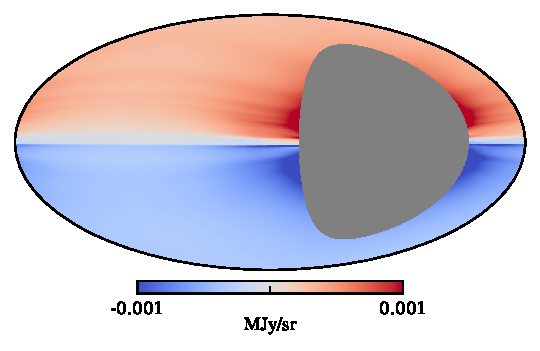
\includegraphics[width=\linewidth]{figs/zodi_obs_diff.pdf}
        \caption{Difference in simulated zodiacal light between an observed at the center of Earth and an observer moved 900km in the positive z-direction from the center of Earth.}
      \label{fig: z}
\end{figure}

\begin{figure}
    \centering
        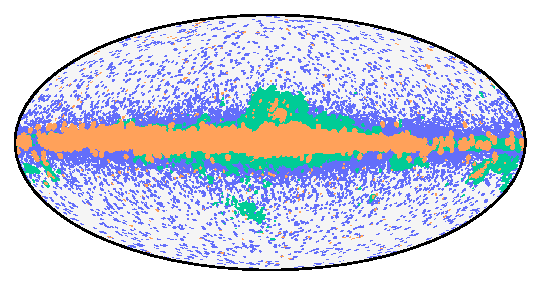
\includegraphics[width=\columnwidth]{figs/mask_zodi_fitting.pdf}
        \caption{Masks applied when fitting zodiacal light parameters for the $2.2\mathrm{\mu m}$, $25\mathrm{\mu m}$ and $240\mathrm{\mu m}$ bands.}
      \label{fig:masks}
\end{figure}

%\subsubsection{Coordinate and geometry}
We allow each zodiacal component to have an offset from the sun
\begin{equation}
    \begin{aligned}
    x_c&= x - x_{0,c}\\
    y_c&= y - y_{0,c}\\
    z_c&= z - z_{0,c}.
    \end{aligned}
\end{equation}
Additionally, each component is inclined at an angle $i$ and have an ascending node $\Omega$, with respect to the ecliptic. This allows us to completely describe the symmetry of a component with respect to its mid-plane with only the two coordinates
\begin{align}
    R_c &= \sqrt{x_c^2 + y_c^2 + z_c^2}\\
    Z_c &= x_c\sin{\Omega_c}\sin{i_c} - y_c \cos{\Omega_c}\sin{i_c} + z_c \cos{i_c}.
\end{align}

\subsection{Emission mechanisms and line-of-sight integration}
%\subsubsection{Thermal emission}

\begin{equation}
    I^\mathrm{Thermal}_{\lambda} = B_\lambda(T).
\end{equation}
\begin{equation}
    T(R) = T_0 R^{-\delta},
\end{equation}
\begin{equation}
    I^\mathrm{Thermal}_{c,\lambda} = E_{c,\lambda} B_\lambda(T(R)).
\end{equation}

%\subsubsection{Scattered light}
\begin{equation}\label{eq: scat_term}
    I^\mathrm{Scattering}_{c, \lambda} = A_{c, \lambda} F_\lambda^\odot(R) \Phi_\lambda(\Theta).
\end{equation}
\begin{equation}
    F_\lambda^\odot(R) = \frac{F_{\lambda,0}^\odot}{R^2},
\end{equation}
\begin{equation}
    \Phi_{\lambda}(\Theta)=N\left[C_{0, \lambda}+C_
    {1, \lambda} \Theta+\mathrm{e}^{C_{2, \lambda} \Theta}\right],
\end{equation}
\begin{equation}
    N = \left[ 2\pi \left( 2 C_{0, \lambda} + \pi C_{1, \lambda} + \frac{\mathrm{e}^{\pi C_{2, \lambda}} + 1}{{C^2_{2, \lambda}} + 1} \right)\right]^{-1}.
\end{equation}

%\subsection{Evaluating the zodiacal light}
\begin{align}
    I^\mathrm{Total}_{c, \lambda} &= I^\mathrm{Scattering}_{c,\lambda} + I^\mathrm{Thermal}_{c,\lambda}\\
    &= A_{c, \lambda} F_\lambda^\odot(R) \Phi_\lambda(\Theta) + \left( 1 - A_{c, \lambda} \right) E_{c,\lambda} B_\lambda(T(R)).
\end{align}

\begin{equation}\label{eq: intensity}
    I_{p,t} = \sum_c \int n_c \left[  A_{c, \lambda} F_\lambda^\odot \Phi_\lambda + \left( 1 - A_{c, \lambda} \right) E_{c,\lambda} B_\lambda \right]\,\mathrm ds,
\end{equation}

\subsection{Reference models}

\subsubsection{DIRBE/Kelsall (K98) model}

%\subsubsection{The diffuse cloud}
\begin{equation}
n_\mathrm{C}(R_\mathrm{C}, Z_\mathrm{C}) = n_{0,\mathrm{C}} R_\mathrm{C}^{-\alpha} f(\zeta_\mathrm{C}).
\end{equation}
%\subsubsection{Asteroidal dust bands}
\begin{equation}
    \begin{aligned}
        n_{\mathrm{B}_j}(R_{\mathrm{B}_j}, Z_{\mathrm{B}_j})=& \frac{3 n_{0, \mathrm{B}_j}}{R_{\mathrm{B}_j}} \exp \left[-\left(\frac{\zeta_{\mathrm{B}_j}}{\delta_{\zeta_{\mathrm B_j}}}\right)^{6}\right]\left[1 + \left(\frac{\zeta_{\mathrm{B}_j}}{\delta_{\zeta_{\mathrm{B}_j}}}\right)^{p_{\mathrm{B}_j}}v^{-1}_{\mathrm{B}_j}\right] \\
        & \times\left\{1-\exp \left[-\left(\frac{R_{\mathrm{B}_j}}{\delta_{R_{\mathrm{B}_j}}}\right)^{20}\right]\right\},
    \end{aligned}
\end{equation}
%\subsubsection{Circumsolar ring and Earth-trailing feature}
\begin{equation}\label{eq: ring}
    n_\mathrm{R}(R_\mathrm{R}, Z_\mathrm{R})=n_{\mathrm{R},0} \exp \left[-\frac{\left(R_\mathrm{R}-R_{0, \mathrm{R}}\right)^2}{\sigma_{\mathrm{R}, r} ^2}-\frac{\left| Z_\mathrm{R} \right|}{\sigma_{\mathrm{R}, z}}\right],
\end{equation}

\begin{equation}\label{eq: feature}
   n_\mathrm{F}(R_\mathrm{F}, Z_\mathrm{F}, \theta_\mathrm{F}) = n_{\mathrm{F}, 0} \exp \left[-\frac{\left(R_\mathrm{F}-R_{\mathrm{F}, 0}\right)^{2}}{\sigma_{\mathrm{F}, r}^{2}}-\frac{\left|Z_\mathrm{F}\right|}{\sigma_{\mathrm{F}, z}}-\frac{\left(\theta_\mathrm{F}-\theta_{\mathrm{F}, 0}\right)^{2}}{\sigma_{\mathrm{F}, \theta }^{2}}\right],
\end{equation}

\subsubsection{Rowan-Robinson and May (RRM) model}
Fill in sections with model components we end up trying/using.
%\subsubsection{The fan}
%\subsubsection{Comets}
%\subsubsection{Narrow bands}
%\subsubsection{Broad bands}
%\subsubsection{Interstellar dust}
%\subsubsection{Circumsolar ring and earth-trailing Feature}


%\subsection{A time-varying foreground}

% HKE: Commented out for now, since it's already shown in the Zodipy paper
%\begin{figure}
%    \centering
%      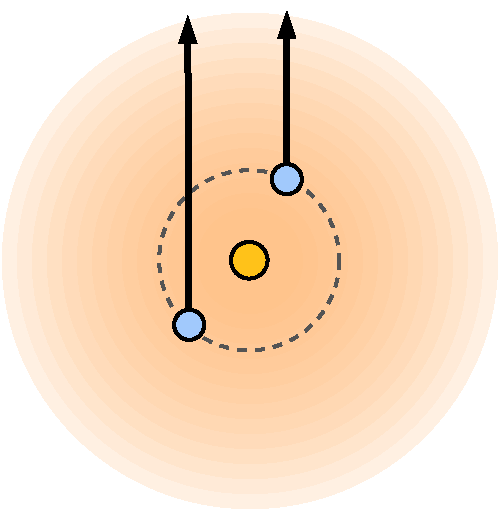
\includegraphics[width=0.7\linewidth]{figs/illustration.pdf}
%      \caption{Illustration showing that the integrated IPD along a line of sight toward a point on the celestial sphere as seen from Earth (blue circles) changes as Earth orbits the Sun (yellow circle).}
%      \label{fig: illustration}
%  \end{figure}

\subsubsection{Survey of zodiacal light parameter variations}

\begin{figure*}
    \centering
    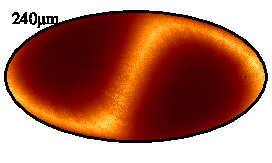
\includegraphics[width=0.22\textwidth]{figs/zodi/zodi_10_tot.pdf}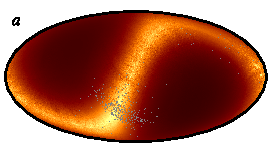
\includegraphics[width=0.22\textwidth]{figs/zodi/zodi_10_a.pdf}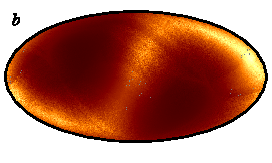
\includegraphics[width=0.22\textwidth]{figs/zodi/zodi_01_b.pdf}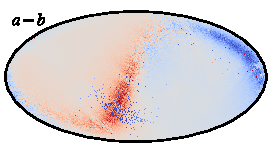
\includegraphics[width=0.22\textwidth]{figs/zodi/zodi_10_a-b.pdf} 
    \vspace{-0.3cm}

    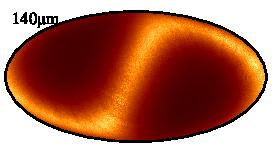
\includegraphics[width=0.22\textwidth]{figs/zodi/zodi_09_tot.pdf}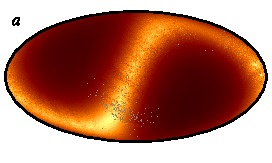
\includegraphics[width=0.22\textwidth]{figs/zodi/zodi_09_a.pdf}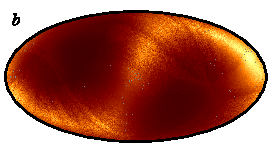
\includegraphics[width=0.22\textwidth]{figs/zodi/zodi_02_b.pdf}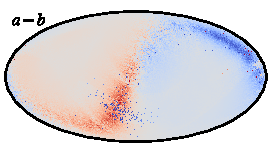
\includegraphics[width=0.22\textwidth]{figs/zodi/zodi_09_a-b.pdf}
    \vspace{-0.3cm}

    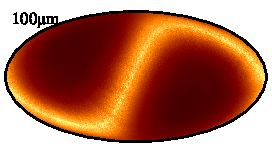
\includegraphics[width=0.22\textwidth]{figs/zodi/zodi_08_tot.pdf}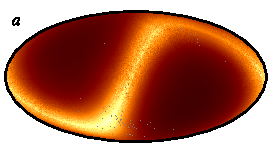
\includegraphics[width=0.22\textwidth]{figs/zodi/zodi_08_a.pdf}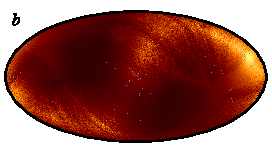
\includegraphics[width=0.22\textwidth]{figs/zodi/zodi_03_b.pdf}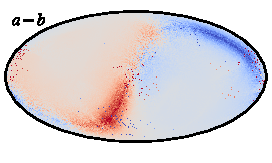
\includegraphics[width=0.22\textwidth]{figs/zodi/zodi_08_a-b.pdf}
    \vspace{-0.3cm}

    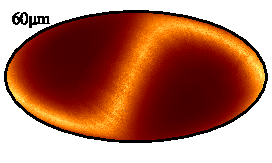
\includegraphics[width=0.22\textwidth]{figs/zodi/zodi_07_tot.pdf}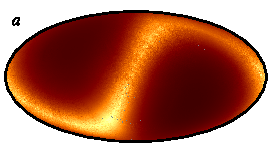
\includegraphics[width=0.22\textwidth]{figs/zodi/zodi_07_a.pdf}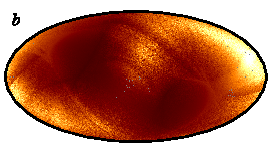
\includegraphics[width=0.22\textwidth]{figs/zodi/zodi_04_b.pdf}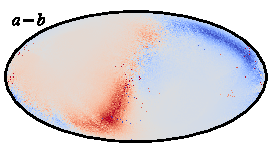
\includegraphics[width=0.22\textwidth]{figs/zodi/zodi_07_a-b.pdf}
    \vspace{-0.3cm}

    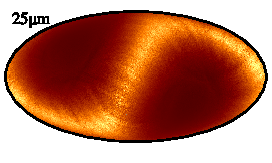
\includegraphics[width=0.22\textwidth]{figs/zodi/zodi_06_tot.pdf}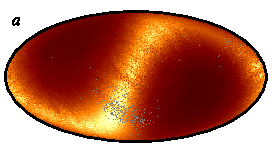
\includegraphics[width=0.22\textwidth]{figs/zodi/zodi_06_a.pdf}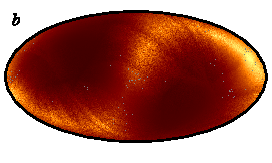
\includegraphics[width=0.22\textwidth]{figs/zodi/zodi_05_b.pdf}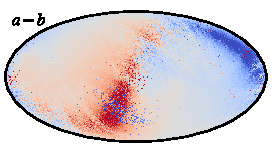
\includegraphics[width=0.22\textwidth]{figs/zodi/zodi_06_a-b.pdf}
    \vspace{-0.3cm}

    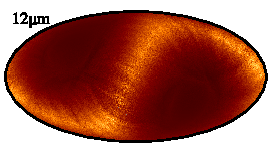
\includegraphics[width=0.22\textwidth]{figs/zodi/zodi_05_tot.pdf}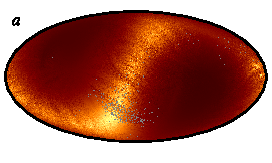
\includegraphics[width=0.22\textwidth]{figs/zodi/zodi_05_a.pdf}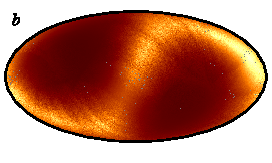
\includegraphics[width=0.22\textwidth]{figs/zodi/zodi_06_b.pdf}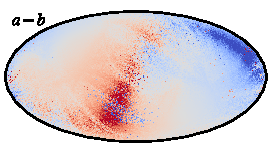
\includegraphics[width=0.22\textwidth]{figs/zodi/zodi_05_a-b.pdf}
    \vspace{-0.3cm}

    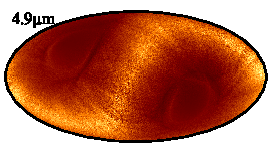
\includegraphics[width=0.22\textwidth]{figs/zodi/zodi_04_tot.pdf}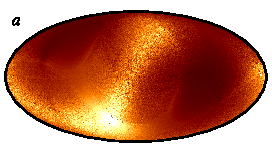
\includegraphics[width=0.22\textwidth]{figs/zodi/zodi_04_a.pdf}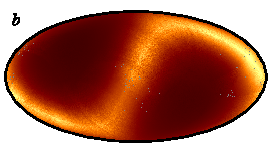
\includegraphics[width=0.22\textwidth]{figs/zodi/zodi_07_b.pdf}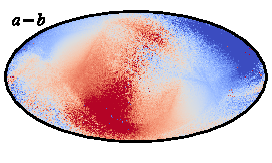
\includegraphics[width=0.22\textwidth]{figs/zodi/zodi_04_a-b.pdf}
    \vspace{-0.3cm}

    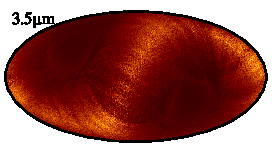
\includegraphics[width=0.22\textwidth]{figs/zodi/zodi_03_tot.pdf}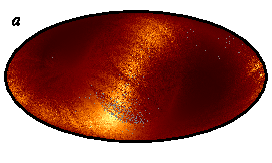
\includegraphics[width=0.22\textwidth]{figs/zodi/zodi_03_a.pdf}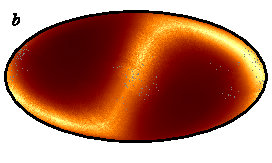
\includegraphics[width=0.22\textwidth]{figs/zodi/zodi_08_b.pdf}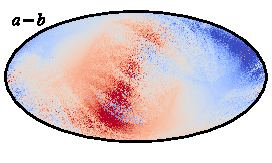
\includegraphics[width=0.22\textwidth]{figs/zodi/zodi_03_a-b.pdf}
    \vspace{-0.3cm}

    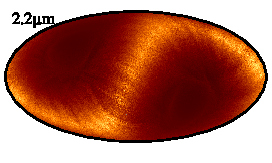
\includegraphics[width=0.22\textwidth]{figs/zodi/zodi_02_tot.pdf}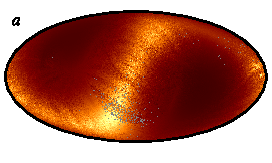
\includegraphics[width=0.22\textwidth]{figs/zodi/zodi_02_a.pdf}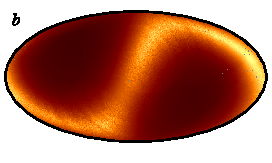
\includegraphics[width=0.22\textwidth]{figs/zodi/zodi_09_b.pdf}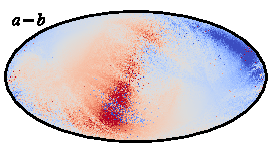
\includegraphics[width=0.22\textwidth]{figs/zodi/zodi_02_a-b.pdf}
    \vspace{-0.3cm}

    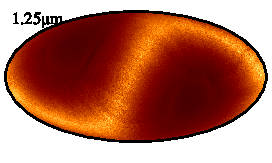
\includegraphics[width=0.22\textwidth]{figs/zodi/zodi_01_tot.pdf}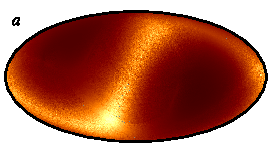
\includegraphics[width=0.22\textwidth]{figs/zodi/zodi_01_a.pdf}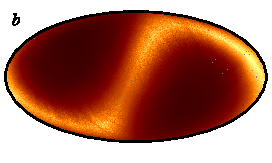
\includegraphics[width=0.22\textwidth]{figs/zodi/zodi_10_b.pdf}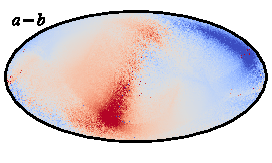
\includegraphics[width=0.22\textwidth]{figs/zodi/zodi_01_a-b.pdf}

    \caption{Zodi frequency maps}
    \label{fig:zodi_freq}
  \end{figure*}

  \begin{figure*}
    \centering
    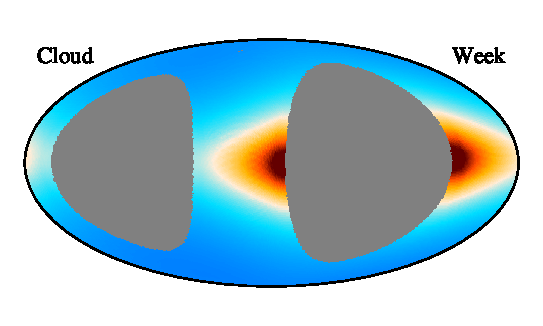
\includegraphics[width=0.9\columnwidth]{figs/zodi_comps/zodi_06_cloud_week.pdf}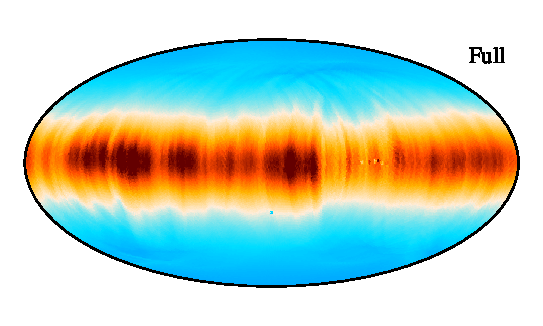
\includegraphics[width=0.9\columnwidth]{figs/zodi_comps/zodi_06_cloud_full.pdf}

    \vspace{-0.6cm}

    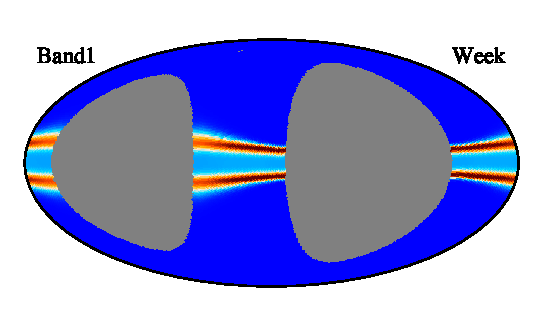
\includegraphics[width=0.9\columnwidth]{figs/zodi_comps/zodi_06_band1_week.pdf}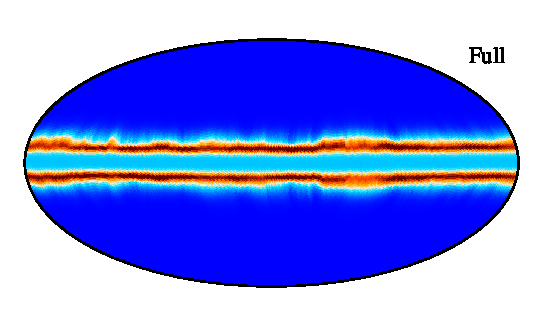
\includegraphics[width=0.9\columnwidth]{figs/zodi_comps/zodi_06_band1_full.pdf}

    \vspace{-0.6cm}

    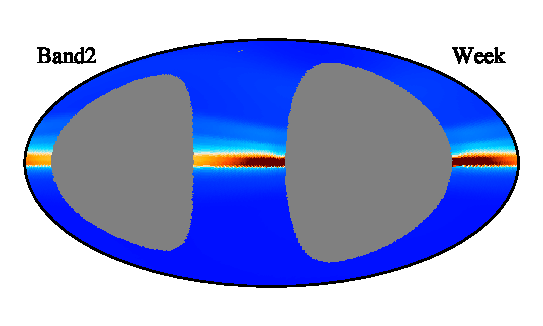
\includegraphics[width=0.9\columnwidth]{figs/zodi_comps/zodi_06_band2_week.pdf}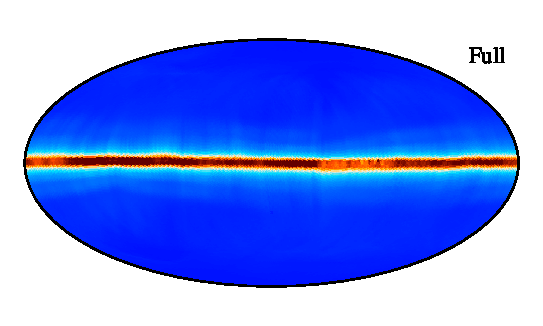
\includegraphics[width=0.9\columnwidth]{figs/zodi_comps/zodi_06_band2_full.pdf}

    \vspace{-0.6cm}

    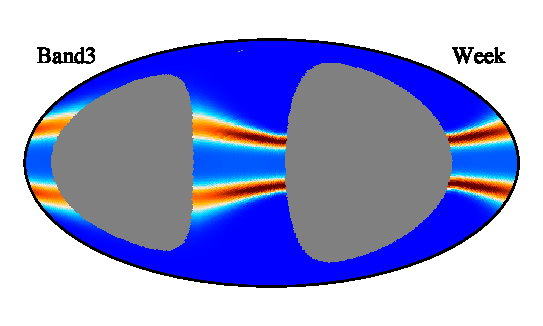
\includegraphics[width=0.9\columnwidth]{figs/zodi_comps/zodi_06_band3_week.pdf}\includegraphics[width=0.9\columnwidth]{figs/zodi_comps/zodi_06_band3_full.pdf}

    \vspace{-0.6cm}

    \includegraphics[width=0.9\columnwidth]{figs/zodi_comps/zodi_06_ring_week.pdf}\includegraphics[width=0.9\columnwidth]{figs/zodi_comps/zodi_06_ring_full.pdf}

    \vspace{-0.6cm}

    \includegraphics[width=0.9\columnwidth]{figs/zodi_comps/zodi_06_feature_week.pdf}\includegraphics[width=0.9\columnwidth]{figs/zodi_comps/zodi_06_feature_full.pdf}

    \caption{week map of comps*}
    \label{fig: comp week}
  \end{figure*}

\begin{figure*}
\centering
\includegraphics[width=0.9\columnwidth]{figs/zodi_comps/zodi_sky_98_week.pdf}\includegraphics[width=0.9\columnwidth]{figs/zodi_comps/zodi_cloud_98_week.pdf}
\vspace{-0.6cm}

\includegraphics[width=0.9\columnwidth]{figs/zodi_comps/zodi_zodi_98_week.pdf}\includegraphics[width=0.9\columnwidth]{figs/zodi_comps/zodi_bands_98_week.pdf}
\vspace{-0.6cm}

\includegraphics[width=0.9\columnwidth]{figs/zodi_comps/zodi_res_98_week.pdf}\includegraphics[width=0.9\columnwidth]{figs/zodi_comps/zodi_ring+feature_98_week.pdf}
\caption{week map of comps*}
\label{fig: K98 week comparison}
\end{figure*}


\begin{figure*}
  \centering
   	\includegraphics[width=0.8\linewidth]{figs/atlas_1_v2.pdf}
  	\caption{Atlas 1}
	\label{fig: atlas1}
\end{figure*}

\begin{figure*}
    \centering
         \includegraphics[width=0.8\linewidth]{figs/atlas_2_v2.pdf}
        \caption{Atlas 2}
      \label{fig: atlas2}
  \end{figure*}


\subsection{DIRBE data}
Discuss data used for sampling of the model. Talk about time-order processing, downsampling, thinning, etc.

%\subsection{Difficulties with sampling and degeneracies in the interplanetary dust model parameters}
See atlases in figure \ref{fig: atlas1} and \ref{fig: atlas2} for degeneracies in the interplanetary dust model parameters.

\subsection{Sampling techniques}

\begin{figure*}
    \centering
    \includegraphics{figs/zodi_params_new.pdf}
    \caption{A subset of the estimated zodiacal light parameters fit in this work.}
    \label{fig: zodi_trace}

\end{figure*}

\begin{figure*}
    \centering
    \includegraphics[width=0.49\linewidth]{figs/maptot_06a_week_minus_full.pdf}
    \includegraphics[width=0.49\linewidth]{figs/maptot_06a_week.pdf}\\
    \includegraphics[width=0.49\linewidth]{figs/mapzodi_06a_week_minus_full.pdf}
    \includegraphics[width=0.49\linewidth]{figs/mapzodi_06a_week.pdf}
    \includegraphics[width=0.49\linewidth]{figs/map_06a_week_minus_full.pdf}
    \includegraphics[width=0.49\linewidth]{figs/map_06a_week.pdf}
    \caption{Illustration of the basic sky maps involved in the zodiacal light fitting algorithms adopted by the DIRBE (\emph{left column}) and \Cosmoglobe\ (\emph{right column}) pipelines for one week of $25\,\mu\mathrm{m}$ observations and adopting the K98 model. The DIRBE pipeline used exclusively differences between weekly and full-season maps, both for the observed signal, $\Delta I_{\nu} \equiv I_{\nu}-\left<I_{\nu}\right>$ (\emph{top left}), and the zodiacal light model, $\Delta Z_{\nu} = Z_{\nu}-\left<Z_{\nu}\right>$ (\emph{middle left}), where brackets indicate full-survey averages. Correspondingly, the final $\chi^2$ is defined through $\Delta I_{\nu} - \Delta Z_{\nu}$ (\emph{bottom left}), and is by constrution only sensitive to time-variable signals. In contrast, the basic data element in \Cosmoglobe\ is the full sky signal, $I_{\nu}$ (\emph{top right}), which is fitted with the full zodiacal light model, $Z_{\nu}$ (\emph{middle right}), both modelled in time-domain. The $\chi^2$ the minimizes minimize the total signal-minus-model residual, $I_{\nu}-Z_{\nu}$ (\emph{bottom right}). The main advantage of the DIRBE approach is insensitivity to stationary sky signals, in particular thermal dust and CIB, while the main advantage of the \Cosmoglobe\ approach is a much higher effective signal-to-noise ratio, both to zodiacal light parameters and zero-levels.}
    \label{fig:week_vs_full}
  \end{figure*}


The approach we will use Gibbs sample each of the model parameters. This means that we propose a change to one model parameter, estimate the zodiacal emission over the full timestream of each ten DIRBE bands, compute a chi-squared and accept/reject. We perform N such proposals before we move on the the next parameter. Since the zodiacal emission is mostly very smooth on the sky, we can afford to downsample the TOD timestream before evaluating the zodiacal emission. For the diffuse cloud and the dust bands we downsample the TODS by X. For the circum-solar ring and the Earth-trailing feature, which are less smooth, and harder to constrain, we downsample the TODS by X. The downsampled TODS are subtracted by the \Cosmoglobe\ skymodel, and recomputed after after each parameter evaluation. 








\clearpage
\section{Reanalysis of the K98 zodiacal light model}



\begin{figure*}
	\centering
	\includegraphics[width=0.8\linewidth]{figs/zodi_diff.pdf}
	\caption{Half-mission model. Columns 1 and 2 are the prediction of the zodiacal emission for each band for the first and second half of the DIRBE mission. Column 3 is the difference between these two columns, and column 4 is the difference between the two zodi-subtracted half-mission maps}
	\label{fig: zodi_HM}
\end{figure*}

\begin{figure*}
    \centering
	 \includegraphics[width=0.8\linewidth]{figs/tod_zodi_residuals.pdf}
	\caption{Data-minus-model residual for \cosmoglobe\ results (CG, black) and the official \citet{k98} model (K98, orange), as a function of ecliptic latitude, Galactic latitude, and Solar elongation. The offset for \cosmoglobe\ and the K98 model are listed on the left and right axes of each row, respectively. The \cosmoglobe\ and K98 values are horizontally offset left and right respectively for clarity.}
      \label{fig: zodi_timestream}
  \end{figure*}

\begin{table*}
    % \renewcommand{\arraystretch}{1.1} % Default value: 1
    \begin{center}
    \small
    \caption{Best fit geometrical interplanetary dust parameters as fit by K98 and us.}
    \label{table:zodi parameters}
    \begin{tabular}{
        l 
        l 
        >{\collectcell{}}r<{\endcollectcell}
        @{${}\pm{}$}
        >{\collectcell{}}l<{\endcollectcell}
        >{\collectcell{}}r<{\endcollectcell}
        @{${}\pm{}$}
        >{\collectcell{}}l<{\endcollectcell}
        >{\collectcell{}}r<{\endcollectcell}
        @{${}\pm{}$}
        >{\collectcell{}}l<{\endcollectcell}
    }
    \hline \hline
    Parameter & Description & \multicolumn{2}{c}{K98} & \multicolumn{2}{c}{Model A} & \multicolumn{2}{c}{Model B} \\
    \hline
    \multicolumn{8}{c}{All zodiacal components}\\
    \hline
    $T_0$ [K]     & Temperature at 1 AU    & \multicolumn{2}{c}{286} & \multicolumn{2}{c}{286} & \multicolumn{2}{c}{286}\\
    $\delta$      & Temperature power-law exponent    & \multicolumn{2}{c}{0.467} & \multicolumn{2}{c}{0.467} & \multicolumn{2}{c}{0.467}\\
    \hline
    \multicolumn{8}{c}{Diffuse cloud}\\
    \hline
    $n_0$ [$10^{-7}$ AU$^{-1}$]     & Density at 1 AU               & 1.13 & 0.0064           & 1.13 & 0.0064         & 1.13 & 0.0064\\
    $\alpha$                        & Radial power-law exponent     & 1.34 & 0.022            & 1.34 & 0.022          & 1.34 & 0.022\\
    $\beta$                         & Vertical shape parameter      & 4.14 & 0.067            & 4.14 & 0.067          & 4.14 & 0.067\\
    $\gamma$                        & Vertical power-law exponent   & 0.942 & 0.025           & 0.942 & 0.025         & 0.942 & 0.025\\
    $\mu$                           & Widening parameter            & 0.189 & 0.014           & 0.189 & 0.014         & 0.189 & 0.014\\
    $i$ [deg]                       & Inclination                   & 2.03 & 0.017            & 2.03 & 0.017          & 2.03 & 0.017\\
    $\Omega$ [deg]                  & Ascending node                & 77.7 & 0.6              & 77.7 & 0.6            & 77.7 & 0.6\\
    $X_0$ [$10^{-3}$ AU]            & x offset from Sun             & 11.9 & 1.1 & 11.9 & 11.9 & 1.1 & 11.9 \\ 
    $Y_0$ [$10^{-3}$ AU]            & y offset from Sun             & 5.48 & 0.77 & 5.48 & 5.48 & 0.77 & 5.48 \\ 
    $Z_0$ [$10^{-3}$ AU]            & z offset from Sun             & 2.15 & 0.43 & 2.15 & 2.15 & 0.43 & 2.15 \\ 
    \hline
    \multicolumn{8}{c}{Asteroidal dust band 1}\\
    \hline
    $n_0$ [$10^{-10}$ AU$^{-1}$]  & Density at 3 AU               & 5.59 & 0.72                 & 5.59 & 0.72               & 5.59 & 0.72\\
    $\delta_{\zeta_{B}}$ [deg]    & Shape parameter               & \multicolumn{2}{c}{8.78}    & \multicolumn{2}{c}{8.78}  & \multicolumn{2}{c}{8.78}\\
    $v_{B}$                       & Shape parameter               & \multicolumn{2}{c}{0.1}     & \multicolumn{2}{c}{0.1}   & \multicolumn{2}{c}{0.1}\\
    $p_{B}$                       & Shape parameter               & \multicolumn{2}{c}{4}       & \multicolumn{2}{c}{4}     & \multicolumn{2}{c}{4}\\
    $i_{B}$ [deg]                 & Inclination                   & \multicolumn{2}{c}{0.56}    & \multicolumn{2}{c}{0.56}  & \multicolumn{2}{c}{0.56}\\
    $\Omega_{B}$ [deg]            & Ascending node                & \multicolumn{2}{c}{80}      & \multicolumn{2}{c}{80}    & \multicolumn{2}{c}{80}\\
    $\delta_{R_{B}}$ [AU]         & Inner radial cutoff           & \multicolumn{2}{c}{1.5}     & \multicolumn{2}{c}{1.5}   & \multicolumn{2}{c}{1.5}\\
    \hline
    \multicolumn{8}{c}{Asteroidal dust band 2}\\
    \hline
    $n_0$ [$10^{-9}$ AU$^{-1}$]   & Density at 3 AU               & 1.99 & 0.128                & 1.99 & 0.128              & 1.99 & 0.128\\
    $\delta_{\zeta_{B}}$ [deg]    & Shape parameter               & \multicolumn{2}{c}{8.78}    & \multicolumn{2}{c}{8.78}  & \multicolumn{2}{c}{8.78}\\
    $v_{B}$                       & Shape parameter               & \multicolumn{2}{c}{0.9}     & \multicolumn{2}{c}{0.9}   & \multicolumn{2}{c}{0.9}\\
    $p_{B}$                       & Shape parameter               & \multicolumn{2}{c}{4}       & \multicolumn{2}{c}{4}     & \multicolumn{2}{c}{4}\\
    $i_{B}$ [deg]                 & Inclination                   & \multicolumn{2}{c}{1.2}     & \multicolumn{2}{c}{1.2}   & \multicolumn{2}{c}{1.2}\\
    $\Omega_{B}$ [deg]            & Ascending node                & \multicolumn{2}{c}{30.3}    & \multicolumn{2}{c}{30.3}  & \multicolumn{2}{c}{30.3}\\
    $\delta_{R_{B}}$ [AU]         & Inner radial cutoff           & \multicolumn{2}{c}{0.94}    & \multicolumn{2}{c}{0.94}  & \multicolumn{2}{c}{0.94}\\
    \hline
    \multicolumn{8}{c}{Asteroidal dust band 3}\\
    \hline
    $n_0$ [$10^{-10}$ AU$^{-1}$]  & Density at 3 AU               & 1.44 & 0.234                & 1.44 & 0.234              & 1.44 & 0.234  \\
    $\delta_{\zeta_{B}}$ [deg]    & Shape parameter               & \multicolumn{2}{c}{15}      & \multicolumn{2}{c}{15}    & \multicolumn{2}{c}{15}\\
    $v_{B}$                       & Shape parameter               & \multicolumn{2}{c}{0.05}    & \multicolumn{2}{c}{0.05}  & \multicolumn{2}{c}{0.05}\\
    $p_{B}$                       & Shape parameter               & \multicolumn{2}{c}{4}       & \multicolumn{2}{c}{4}     & \multicolumn{2}{c}{4}\\
    $i_{B}$ [deg]                 & Inclination                   & \multicolumn{2}{c}{0.8}     & \multicolumn{2}{c}{0.8}   & \multicolumn{2}{c}{0.8}\\
    $\Omega_{B}$ [deg]            & Ascending node                & \multicolumn{2}{c}{80}      & \multicolumn{2}{c}{80}    & \multicolumn{2}{c}{80}\\
    $\delta_{R_{B}}$ [AU]         & Inner radial cutoff           & \multicolumn{2}{c}{1.5}     & \multicolumn{2}{c}{1.5}   & \multicolumn{2}{c}{1.5}\\
    \hline
    \multicolumn{8}{c}{Circumsolar Ring}\\
    \hline
    $n_\mathrm{SR}$ [$10^{-8}$ AU$^{-1}$]   & Density at 1 AU           & 1.83 & 0.127              & 1.83 & 0.127              & 1.83 & 0.127\\
    $R_\mathrm{SR}$ [AU]                    & Radius of peak density    & 1.03 & 0.00016            & 1.03 & 0.00016            & 1.03 & 0.00016\\
    $\sigma_\mathrm{rSR}$ [AU]              & Radial dispersion         & \multicolumn{2}{c}{0.025} & \multicolumn{2}{c}{0.025} & \multicolumn{2}{c}{0.025}\\
    $\sigma_\mathrm{zSR}$ [AU]              & Vertical dispersion       & 0.054 & 0.0066            & 0.054 & 0.0066            & 0.054 & 0.0066\\
    $i_\mathrm{RB}$ [deg]                   & Inclination               & 0.49  & 0.063             & 0.49  & 0.063             & 0.49  & 0.063\\
    $\Omega_\mathrm{RB}$ [deg]              & Ascending node            & 22.3  & 0.0014            & 22.3 & 0.0014             & 22.3 & 0.0014\\
    \hline
    \multicolumn{8}{c}{Trailing Feature}\\
    \hline
    $n_\mathrm{TB}$ [$10^{-8}$ AU$^{-1}$]   & Density at 1 AU                   & 1.9 & 0.142 & 1.9 & 0.142 & 1.9 & 0.142\\
    $R_\mathrm{TB}$ [AU]                    & Radius of peak density            & 1.06 & 0.011 & 1.06 & 0.011 & 1.06 & 0.011\\
    $\sigma_\mathrm{rTB}$ [AU]              & Radial dispersion                 &  0.10 & 0.0097 & 0.10 & 0.0097 & 0.10 & 0.0097\\
    $\sigma_\mathrm{zTB}$ [AU]              & Vertical dispersion               & 0.091 &  0.013 & 0.091 &  0.013 & 0.091 &  0.013\\
    $\theta_\mathrm{TB}$ [deg]              & Longitude with respect to Earth   & \multicolumn{2}{c}{-10} & \multicolumn{2}{c}{-10} & \multicolumn{2}{c}{-10}\\
    $\sigma_\mathrm{\theta TB}$ [deg]       & Longitude dispersion              & 12.1 & 3.4 & 12.1 & 3.4 & 12.1 & 3.4\\
    \hline    
    \end{tabular}
    \end{center}
\end{table*}


\begin{table*}
    % \renewcommand{\arraystretch}{1.1} % Default value: 1
    \begin{center}
    \small
    \caption{Best fit zodiacal light source parameters from this analysis and the K98 model.}
    \label{table:zodi parameters}
    \begin{tabular}{
        l 
        >{\collectcell\Num}r<{\endcollectcell}
        @{${}\pm{}$}
        >{\collectcell\Num}l<{\endcollectcell}
        >{\collectcell\Num}r<{\endcollectcell}
        @{${}\pm{}$}
        >{\collectcell\Num}l<{\endcollectcell}
        >{\collectcell\Num}r<{\endcollectcell}
        @{${}\pm{}$}
        >{\collectcell\Num}l<{\endcollectcell}
        >{\collectcell\Num}r<{\endcollectcell}
        @{${}\pm{}$}
        >{\collectcell\Num}l<{\endcollectcell}
        >{\collectcell\Num}r<{\endcollectcell}
        @{${}\pm{}$}
        >{\collectcell\Num}l<{\endcollectcell}
        >{\collectcell\Num}r<{\endcollectcell}
        @{${}\pm{}$}
        >{\collectcell\Num}l<{\endcollectcell}
    }
    \hline \hline
    Channel [$\mu$m] & \multicolumn{2}{c}{Diffuse Cloud} & \multicolumn{2}{c}{Dust band 1} & \multicolumn{2}{c}{Dust band 2} & \multicolumn{2}{c}{Dust band 3} & \multicolumn{2}{c}{Circumsolar ring} & \multicolumn{2}{c}{Trailing feature} \\
    \hline
    \multicolumn{13}{c}{Emissivity}\\
    \hline
    3.5  & 1.66 & 0.088 & \multicolumn{2}{c}{1} & \multicolumn{2}{c}{1} & \multicolumn{2}{c}{1} & \multicolumn{2}{c}{1} & \multicolumn{2}{c}{1} \\
    4.9  & 0.997 & 0.0036 & \multicolumn{2}{c}{1} & \multicolumn{2}{c}{1} & \multicolumn{2}{c}{1} & \multicolumn{2}{c}{1} & \multicolumn{2}{c}{1} \\
    12  & 0.958 & 0.002 & \multicolumn{2}{c}{1} & \multicolumn{2}{c}{1} & \multicolumn{2}{c}{1} & \multicolumn{2}{c}{1} & \multicolumn{2}{c}{1} \\
    25  & \multicolumn{2}{c}{1} & \multicolumn{2}{c}{1} & \multicolumn{2}{c}{1} & \multicolumn{2}{c}{1} & \multicolumn{2}{c}{1} & \multicolumn{2}{c}{1} \\
    60  & 0.733 & 0.0055 & \multicolumn{2}{c}{1} & \multicolumn{2}{c}{1} & \multicolumn{2}{c}{1} & \multicolumn{2}{c}{1} & \multicolumn{2}{c}{1} \\
    100  & 0.647 & 0.012 & \multicolumn{2}{c}{1} & \multicolumn{2}{c}{1} & \multicolumn{2}{c}{1} & \multicolumn{2}{c}{1} & \multicolumn{2}{c}{1} \\
    140  & \multicolumn{2}{c}{1} & \multicolumn{2}{c}{1} & \multicolumn{2}{c}{1} & \multicolumn{2}{c}{1} & \multicolumn{2}{c}{1} & \multicolumn{2}{c}{1} \\
    240  & \multicolumn{2}{c}{1} & \multicolumn{2}{c}{1} & \multicolumn{2}{c}{1} & \multicolumn{2}{c}{1} & \multicolumn{2}{c}{1} & \multicolumn{2}{c}{1} \\
    \hline
    \multicolumn{13}{c}{Albedo}\\
    \hline
    1.25  & \multicolumn{2}{c}{1} & \multicolumn{2}{c}{1} & \multicolumn{2}{c}{1} & \multicolumn{2}{c}{1} & \multicolumn{2}{c}{1} & \multicolumn{2}{c}{1} \\
    2.2  & \multicolumn{2}{c}{1} & \multicolumn{2}{c}{1} & \multicolumn{2}{c}{1} & \multicolumn{2}{c}{1} & \multicolumn{2}{c}{1} & \multicolumn{2}{c}{1} \\
    3.5  & \multicolumn{2}{c}{1} & \multicolumn{2}{c}{1} & \multicolumn{2}{c}{1} & \multicolumn{2}{c}{1} & \multicolumn{2}{c}{1} & \multicolumn{2}{c}{1} \\
    \end{tabular}
    \end{center}
\end{table*}


\clearpage
\section{Extended zodiacal light models}

\subsection{Generalized K98 modelling}

\subsection{RRM modelling}

%\subsection{Interplanetary dust model}
Describe the model components used and tabulate all parameters fit.

%\subsection{Spectral parameters (emissivities / albedos)}

%\subsection{Zodi subtracted DIRBE maps and timestreams}

\section{Conclusions}


\begin{acknowledgements}
 The current work has received funding from the European
  Union’s Horizon 2020 research and innovation programme under grant
  agreement numbers 819478 (ERC; \textsc{Cosmoglobe}) and 772253 (ERC;
  \textsc{bits2cosmology}). Some of the results in this paper have been derived using the HEALPix \citep{HEALPIX} package.
  We acknowledge the use of the Legacy Archive for Microwave Background Data
  Analysis (LAMBDA), part of the High Energy Astrophysics Science Archive Center
  (HEASARC). HEASARC/LAMBDA is a service of the Astrophysics Science Division at
  the NASA Goddard Space Flight Center.  
\end{acknowledgements}


%-------------------------------------------------------------
%                                       Table with references 
%-------------------------------------------------------------
%

\bibliographystyle{aa}
\bibliography{references}
\end{document}
%%%% End of aa.dem
